% InkCloser architecture overview (Figure 2).
% Compile: pdflatex fig_diagram.tex  ->  fig_diagram.pdf
% Needs thumb_in.png, thumb_out.png, thumb_gt.png, thumb_hole.png in the same folder.
\documentclass[tikz,border=4pt]{standalone}
\usepackage{amsmath,amssymb}
\usetikzlibrary{positioning,calc,arrows.meta,shapes.misc,fit,backgrounds}

% ---------------------------------------------------------------- colours
\definecolor{encC}{HTML}{9ECAE9}   % gated-conv encoder stages
\definecolor{encD}{HTML}{2F6FA8}
\definecolor{decC}{HTML}{FDD0A2}   % decoder stages
\definecolor{decD}{HTML}{C8681C}
\definecolor{attC}{HTML}{D9C8EC}   % transformer
\definecolor{attD}{HTML}{6A4C93}
\definecolor{dilC}{HTML}{B9E3C6}   % dilated residual stack
\definecolor{dilD}{HTML}{2E8B57}
\definecolor{lossC}{HTML}{FBE3E3}
\definecolor{lossD}{HTML}{B22222}
\definecolor{skipD}{HTML}{555555}

\tikzset{
  >={Stealth[length=4pt,width=3.2pt]},
  flow/.style={->,line width=0.7pt,black!80},
  down/.style={->,line width=0.8pt,encD},
  up/.style={->,line width=0.8pt,decD},
  skip/.style={->,line width=0.6pt,skipD,densely dashed},
  train/.style={->,line width=0.7pt,lossD,dash pattern=on 2.5pt off 1.5pt},
  cat/.style={circle,draw=black!70,fill=white,line width=0.6pt,inner sep=0pt,minimum size=2.6mm,
              path picture={\draw[black!70,line width=0.5pt]
                ($(path picture bounding box.north)+(0,-0.45mm)$)--($(path picture bounding box.south)+(0,0.45mm)$)
                ($(path picture bounding box.west)+(0.45mm,0)$)--($(path picture bounding box.east)+(-0.45mm,0)$);}},
  wide/.style={rounded corners=1.5pt,line width=0.6pt,align=center,font=\scriptsize,inner sep=2pt},
  dim/.style={font=\tiny,text=black!75,align=center,inner sep=1pt},
  lab/.style={font=\scriptsize,align=center,inner sep=1pt},
}

% \stage{name}{x}{y}{width}{height}{fill}{draw}
\newcommand{\stage}[7]{%
  \node[draw=#7,fill=#6,line width=0.6pt,rounded corners=0.8pt,
        minimum width=#4cm,minimum height=#5cm,inner sep=0pt] (#1) at (#2,#3) {};}

\renewcommand{\tiny}{\fontsize{5.6}{6.4}\selectfont}
\begin{document}
\begin{tikzpicture}

% ------------------------------------------------------------ geometry
% level k <-> resolution 896/2^k ; channels 16*2^k
\def\dy{1.15}   % vertical distance between resolution levels
\def\dx{0.6}    % encoder step
\def\doff{0.6}  % decoder block sits this far below its level line

% ============================================================ ENCODER
\foreach \k/\c/\r in {0/16/896,1/32/448,2/64/224,3/128/112,4/256/56,5/512/28}{
  \pgfmathsetmacro{\x}{\k*\dx}
  \pgfmathsetmacro{\y}{-\k*\dy}
  \pgfmathsetmacro{\w}{0.14+0.05*\k}
  \pgfmathsetmacro{\h}{0.75-0.09*\k}
  \stage{E\k}{\x}{\y}{\w}{\h}{encC}{encD}
  \ifnum\k=0 \node[dim,anchor=south] at ($(E\k.north)+(0,0.02)$) {$\r^2$\\[-1pt]\c};
  \else \node[dim,anchor=east] at ($(E\k.west)+(-0.04,0)$) {$\r^2$\\[-1pt]\c};\fi
}
\foreach \k [evaluate=\k as \n using int(\k+1)] in {0,...,4}{
  \draw[down] (E\k.south) -- (E\n.north);
}

% ============================================================ INPUT
\node[draw=black!50,line width=0.4pt,inner sep=0pt] (inp) at (-2.05,0)
  {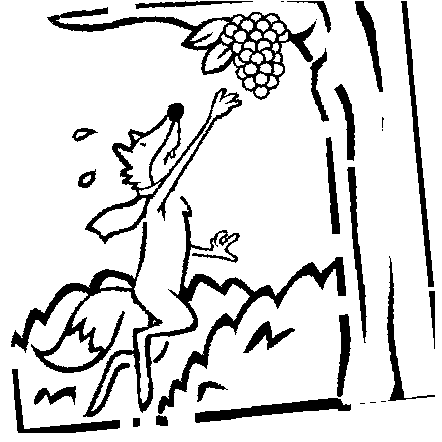
\includegraphics[width=1.75cm]{thumb_in.png}};
\node[lab,above=1pt of inp] {Corrupted input $X$};
\node[dim,below=1pt of inp] {$896\times896\times1$, no mask};
\draw[flow] (inp.east) -- (E0.west);

% ============================================================ BOTTLENECK (28x28)
\node[wide,draw=attD,fill=attC,minimum width=2.9cm,minimum height=0.8cm,anchor=west]
  (batt) at ($(E5.east)+(0.4,0)$)
  {\textbf{Transformer}\,$\times$6\\[-2pt]
   {\tiny $28^2{=}784$ tokens, $d{=}512$, 8 heads}\\[-2pt]{\tiny + 2D sinusoidal pos.\ emb.}};
\draw[flow] (E5.east) -- (batt.west);

% ============================================================ MID-LEVEL CONTEXT (56x56 skip)
\node[wide,draw=dilD,fill=dilC,minimum width=1.85cm,minimum height=0.66cm,anchor=west]
  (dil) at ($(E4.east)+(0.3,0)$)
  {\textbf{Dilated res.}\,$\times$5\\[-2pt] {\tiny dilation 1,\,2,\,4,\,8,\,16}};
\node[wide,draw=attD,fill=attC,minimum width=2.05cm,minimum height=0.66cm,right=0.25cm of dil]
  (matt) {\textbf{Transformer}\,$\times$3\\[-2pt] {\tiny $56^2{=}3136$ tok., $d{=}256$}};
\draw[flow] (E4.east) -- (dil.west);
\draw[flow] (dil.east) -- (matt.west);
% fp32 note spanning both attention modules
\node[font=\tiny,text=attD,anchor=north] at (batt.south) {both attention modules run in fp32};

% ============================================================ DECODER
% D1..D5 at levels 4..0 ; concat nodes C4..C0 on the level lines
\pgfmathsetmacro{\xdone}{8.75}
\foreach \i/\k/\c/\r in {1/4/256/56,2/3/128/112,3/2/64/224,4/1/32/448,5/0/16/896}{
  \pgfmathsetmacro{\x}{\xdone+(\i-1)*0.7}
  \pgfmathsetmacro{\y}{-\k*\dy}
  \pgfmathsetmacro{\w}{0.14+0.05*\k}
  \pgfmathsetmacro{\h}{0.75-0.09*\k}
  \stage{D\i}{\x}{\y-\doff}{\w}{\h}{decC}{decD}
  \node[cat] (C\k) at (\x,\y) {};
  \draw[flow] (D\i.north) -- (C\k.south);
  \node[dim,anchor=west] at ($(D\i.east)+(0.03,0)$) {$\r^2$\\[-1pt]\c};
}
% transposed-conv upsampling between levels
\draw[up] (batt.east) -| (D1.south);
\foreach \k/\i in {4/2,3/3,2/4,1/5}{ \draw[up] (C\k.east) -- (D\i.west); }

% ------------------------------------------------------------ skip connections
\draw[skip] (matt.east) -- (C4.west);
\foreach \k in {0,...,3}{ \draw[skip] (E\k.east) -- (C\k.west); }
\node[font=\tiny,text=skipD,anchor=south] at ($(E0.east)!0.5!(C0.west)$) {skip connection (copy \& concatenate)};

% ============================================================ HEAD & OUTPUT
\node[wide,draw=decD,fill=decC,minimum height=0.75cm,minimum width=0.95cm,anchor=west]
  (head) at ($(C0.east)+(0.32,0)$) {Conv\\[-1pt]$\times3$\\[-1pt]$\rightarrow$1};
\draw[flow] (C0.east) -- (head.west);

\node[draw=black!50,line width=0.4pt,inner sep=0pt,anchor=west] (out) at ($(head.east)+(1.35,0)$)
  {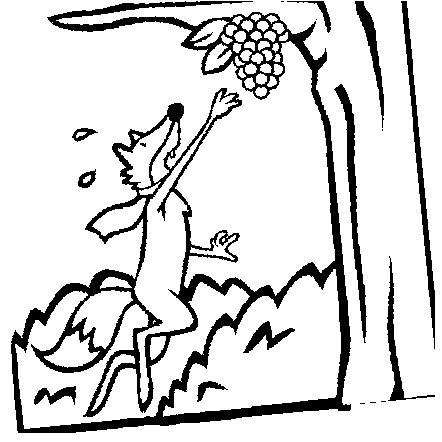
\includegraphics[width=1.75cm]{thumb_out.png}};
\node[lab,above=1pt of out] {Restored output $\hat Y$};
\node[dim,below=1pt of out] {$896\times896\times1$};
\draw[flow] (head.east) -- node[above,font=\tiny,align=center]{sigmoid\\[-1pt](inference)} (out.west);

% ============================================================ LOSS (training only)
\node[draw=lossD,fill=lossC,rounded corners=2pt,line width=0.6pt,dash pattern=on 3pt off 1.5pt,
      minimum width=5.1cm,minimum height=2.2cm,anchor=north east] (lossbox)
      at ($(out.south east)+(0.3,-2.0)$) {};
\node[font=\scriptsize\bfseries,text=lossD,anchor=north west] at ($(lossbox.north west)+(0.08,-0.05)$)
  {Training loss};
\node[inner sep=0pt,draw=black!40,line width=0.3pt,anchor=north west] (gt) at ($(lossbox.north west)+(0.18,-0.42)$)
  {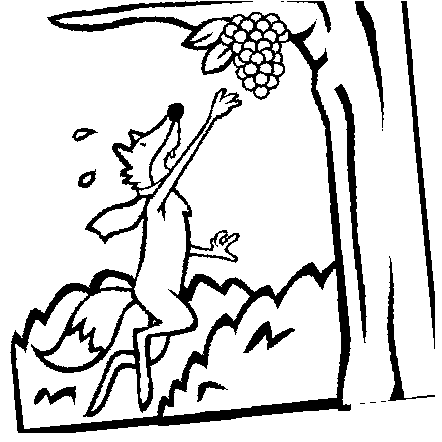
\includegraphics[width=1.05cm]{thumb_gt.png}};
\node[dim,below=0.5pt of gt] {target $Y$};
\node[inner sep=0pt,draw=black!40,line width=0.3pt,right=0.45cm of gt] (hm)
  {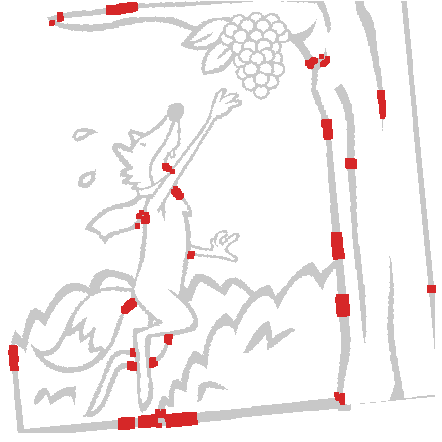
\includegraphics[width=1.05cm]{thumb_hole.png}};
\node[dim,below=0.5pt of hm,align=center] {hole mask $h$\\[-1pt]from $(X,Y)$};
\node[font=\scriptsize,anchor=north west,align=left,inner sep=0pt] at ($(hm.north east)+(0.2,0.02)$)
  {$\mathcal{L}=\;\mathcal{L}_{\mathrm{bce}}^{\lambda_h=3}$\\[1pt]
   $\phantom{\mathcal{L}=}\;+\;\mathcal{L}_{\mathrm{dice}}$\\[1pt]
   $\phantom{\mathcal{L}=}\;+\;0.5\,\mathcal{L}_{\mathrm{gap\,dice}}^{\,r=7}$};
\draw[train] (head.south) -- node[pos=0.55,right,font=\tiny,text=lossD,align=left]{logits\\[-1pt](training)}
  (head.south |- lossbox.north);

% ============================================================ GATED-CONV INSET
\begin{scope}[shift={(-2.95,-3.55)}]
  \node[font=\scriptsize\bfseries,anchor=west] at (0,0.42) {Gated convolution};
  \node[draw=encD,fill=encC!60,rounded corners=1pt,font=\tiny,minimum width=1.0cm,minimum height=0.32cm] (cf) at (1.15,0) {Conv$_f$};
  \node[draw=encD,fill=encC!60,rounded corners=1pt,font=\tiny,minimum width=1.0cm,minimum height=0.32cm] (cg) at (1.15,-0.55) {Conv$_g$};
  \node[draw=encD,fill=white,rounded corners=1pt,font=\tiny,minimum height=0.32cm,inner sep=1.5pt,right=0.18cm of cg] (sg) {$\sigma$};
  \node[circle,draw=black!70,inner sep=0pt,minimum size=2.6mm,font=\tiny] (mul) at ($(sg.east)+(0.42,0.275)$) {$\odot$};
  \node[font=\tiny] (xin) at (0.05,-0.275) {$x$};
  \draw[flow,line width=0.5pt] (xin.east) -- ++(0.12,0) |- (cf.west);
  \draw[flow,line width=0.5pt] (xin.east) -- ++(0.12,0) |- (cg.west);
  \draw[flow,line width=0.5pt] (cg.east) -- (sg.west);
  \draw[flow,line width=0.5pt] (cf.east) -| (mul.north);
  \draw[flow,line width=0.5pt] (sg.east) -| (mul.south);
  \draw[flow,line width=0.5pt] (mul.east) -- ++(0.3,0) node[right,font=\tiny]{$y$};
  \node[font=\tiny,anchor=north west,align=left,text=black!75] at (0,-0.85)
    {$y=\mathrm{Conv}_f(x)\odot\sigma(\mathrm{Conv}_g(x))$\\[-1pt]
     soft per-pixel gate on unreliable input};
\end{scope}

% ============================================================ LEGEND
\begin{scope}[font=\tiny]
  \node[draw=encD,fill=encC,minimum width=0.28cm,minimum height=0.22cm,inner sep=0pt] (l1) at (-2.8,-6.95) {};
  \node[anchor=west,align=left] (t1) at (l1.east) {Encoder stage: 2$\times$ gated conv\\[-1pt]+ GroupNorm + ReLU};
  \node[draw=decD,fill=decC,minimum width=0.28cm,minimum height=0.22cm,inner sep=0pt,right=0.4cm of t1] (l2) {};
  \node[anchor=west,align=left] (t2) at (l2.east) {Decoder stage: transposed conv\\[-1pt]+ conv, GroupNorm + ReLU};
  \coordinate[right=0.4cm of t2] (a3);
  \draw[down] ($(a3)+(0,0.12)$) -- ($(a3)+(0.3,-0.12)$);
  \node[anchor=west,align=left] (t3) at ($(a3)+(0.33,0)$) {gated conv $4{\times}4$,\\[-1pt]stride 2 ($\downarrow$2)};
  \coordinate[right=0.4cm of t3] (a4);
  \draw[up] ($(a4)+(0,-0.12)$) -- ($(a4)+(0.3,0.12)$);
  \node[anchor=west,align=left] (t4) at ($(a4)+(0.33,0)$) {transposed conv $4{\times}4$,\\[-1pt]stride 2 ($\uparrow$2)};
  \node[cat,right=0.4cm of t4] (l5) {};
  \node[anchor=west] (t5) at (l5.east) {channel concat};
  \node[draw=black!70,minimum width=0.15cm,minimum height=0.3cm,inner sep=0pt,right=0.4cm of t5] (l6) {};
  \node[anchor=west,align=left] at (l6.east) {resolution$^2$ /\\[-1pt]channels};
\end{scope}

\end{tikzpicture}
\end{document}
